\chapter[Demo]{A Demonstration of Some LaTeX Features}
\label{ch: demo}

\section{Basics}
\label{sec:Basics}

Some of the \textbf{greatest}
discoveries in \underline{science}
were made by \textbf{\textit{accident}}.

Some of the greatest \emph{discoveries}
in science
were made by accident.

\textit{Some of the greatest \emph{discoveries}
    in science
    were made by accident.}

\textbf{Some of the greatest \emph{discoveries}
    in science
    were made by accident.}

\section{Cross References}
\label{sec:Cross References}

\LaTeX\ has elaborated cross references like e.g.
% use \vref because it also memtions the page number
\begin{compactitem}[$\blacksquare$]
    \item \vref{fig:An elaborated demonstration of pgfplot capabilities}
    \item Did you know that \vpageref{fig:An elaborated demonstration of pgfplot capabilities} we find
    \cref{fig:An elaborated demonstration of pgfplot capabilities}
    \item \vref{sec:Including Figures}
    \item \vref{ch: A Second Demonstration of LaTeX Features}
    \item \vref{sec:Tables}
\end{compactitem}

See \url{https://tex.stackexchange.com/a/83051/144487} for what you can do with it

\pagebreak

\section{Enumerations}
\label{sec:Enumerations}

You can define keywords

\begin{enumerate}[{Example} a)]
    \item Internal combustion optimization
    \item Exhaust gas aftertreatment
    \item Friction reduction
\end{enumerate}

or

\begin{enumerate}[(i)]
    \item Internal combustion optimization
    \item Exhaust gas aftertreatment
    \item Friction reduction
\end{enumerate}


\section{Including Figures}
\label{sec:Including Figures}

\lipsum[1]

\begin{figure}[!h]
    \centering
    % note that height and width are determined *before* rotation,
    % therefore the height is the width after rotation 
    % The png was generated using 
    % rsvg-convert -w 300 fh-logo-right.svg -o fh-logo-right.png
    
\includegraphics[height=0.5\textwidth, angle=270]{fh-logo-right}
    \caption[The FH Aachen Logo]{The logo of Fachhochschule Aachen}
    \label{fh-logo}
\end{figure}

It is also possible to adjust the position of the image and crop it, thereby offering the inclusion of only parts of an image (see e.g. \url{https://texblog.org/2012/02/23/crop-figures-with-includegraphics/}):

\begin{figure}[!h]
    \centering
    % Note that the file ending has to be mentioned explicitly, 
    % otherwise the file thesis.pdf would be tried to be included, 
    % and not images/thesis.png
    % The scheme is: trim=left bottom right top, clip
    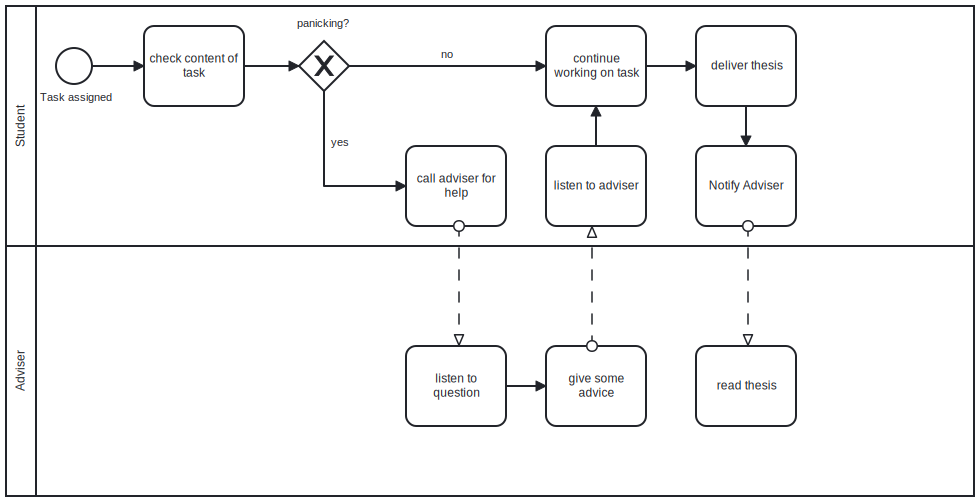
\includegraphics[trim=50 300 200 10,clip,width=\textwidth]{thesis.png}
    \caption[Some cropped image]{A cropped version of \vref{The complete image}}
    \label{cropped image}
\end{figure}

The complete figure is

\begin{figure}[!h]
    \centering
    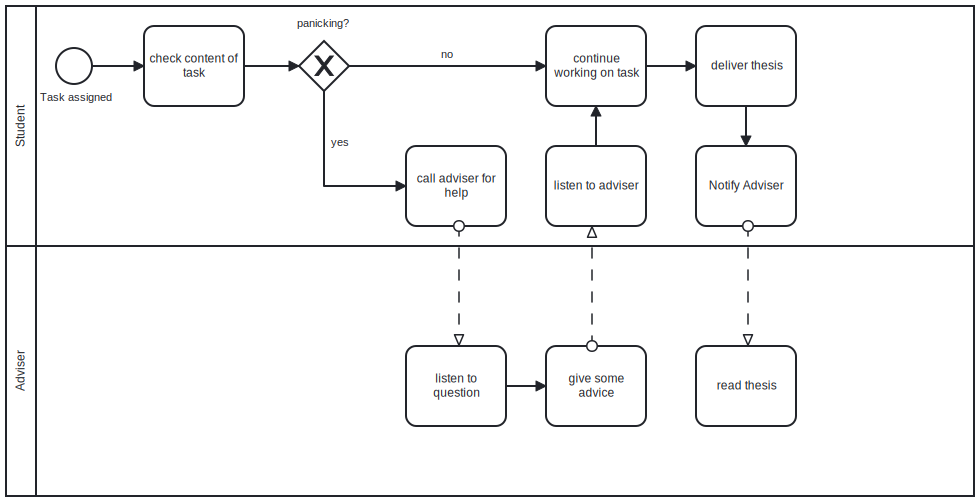
\includegraphics[width=\textwidth]{thesis.png}
    \caption{The complete image}
    \label{The complete image}
\end{figure}



% clearpage enfoeces all floating objects like tables and figures to be rendered before starting a new section or chapter

\clearpage

\section{Formulas}
\label{sec:Formulas}

Subscripts in math mode are written as $a_b$ and superscripts are written as $a^b$. These can be combined an nested to write expressions such as

\begin{equation}
    T^{i_1 i_2 \dots i_p}_{j_1 j_2 \dots j_q} = T(x^{i_1},\dots,x^{i_p},e_{j_1},\dots,e_{j_q})
    \label{a complicated formula 1}
\end{equation}

We write integrals using $\int$ and fractions using $\frac{a}{b}$. Limits are placed on integrals using superscripts and subscripts:

\begin{equation}
    \int_0^1 \frac{dx}{e^x} =  \frac{e-1}{e}
\end{equation}

Lower case Greek letters are written as $\omega$ $\delta$ etc. while upper case Greek letters are written as $\Omega$ $\Delta$.

Mathematical operators are prefixed with a backslash as $\sin(\beta)$, $\cos(\alpha)$, $\log(x)$ etc.

    {
        \small
        \begin{subequations}
            \begin{align}
                % ======================================================================
                % Massenbilanz
                \label{Bilanzgleichungen in konservativer differentieller Form a}
                              & \pfrac{\rho}{t}           & + \      & \diverg \left( \rho \tvec{v} \right) &  &  &  &  & =
                \quad         & 0 \qquad
                \\[.5em]
                % ======================================================================
                % Impulsbilanz
                \label{Bilanzgleichungen in konservativer differentieller Form b}
                              & \pfrac{(\rho\tvec{v})}{t}
                              & + \                       &
                \diverg \left( \rho \tvec{v} \circ \tvec{v} \right)
                              & - \                       &
                \diverg \tenstress
                              & - \                       &
                \rho \tvec{b} & = \quad                   & 0 \qquad
                \\[.5em]
                % ======================================================================
                % Energiebilanz
                \label{Bilanzgleichungen in konservativer differentieller Form c}
                              & \pfracbig{                                                                                  %
                    \left(
                    \rho \left[ e + \frac{\tvec{v}^2}{2} \right]
                    \right)}{t}
                              & + \                       &
                \diverg \left(
                \rho \left[ e + \frac{\tvec{v}^2}{2} \right] \tvec{v}
                \right)
                              & - \                       &
                \diverg \left( \tvec{v} \tenstress - \tvec{q} \right)
                              & - \                       &
                \rho \left( \tvec{v} \tvec{b} - \tvec{q_b} \right)
                              & = \quad                   & 0 \qquad
            \end{align}
        \end{subequations}
    }

\clearpage

\chapter[Demo 2]{A Second Demonstration of LaTeX Features}
\label{ch: A Second Demonstration of LaTeX Features}

\section{Tables}
\label{sec:Tables}

\subsection{Using \LaTeX\ package \texttt{tabularx}}
\label{sec: using LaTeX package tabularx}

{
    \newcolumntype{L}[1]{>{\hsize=#1\hsize\raggedright\arraybackslash}X}%
    \newcolumntype{R}[1]{>{\hsize=#1\hsize\raggedleft\arraybackslash}X}%
    \newcolumntype{C}[2]{>{\hsize=#1\hsize\columncolor{#2}\centering\arraybackslash}X}%

    \begin{table}[htbp]
        \centering
        % Note that labels should be on top for tables 
        \caption{A simple table with paragraphs}
        \label{tab: A simple table with paragraphs}%
        \begin{tabularx}{\textwidth}{ | L{2} | R{0.5} | R{1} | C{0.5}{green} | }
            \hline
            This could be a longer text and that is OK because this is what tabularx was made for & label 2 & label 3 & item x \\
            \hline
            item 1                                                                                & item 2  & item 3  & item 4 \\
            \hline
        \end{tabularx}
    \end{table}%
}

\subsection{Using a Regular \LaTeX\ \texttt{tabular} Environment}
\label{sec: Using a Regular LaTeX tabularx Environment}

A table generated with the Excel plugin Excel2LaTeX.
Please note how we use an \texttt{adjustbox} to enforce the table to fit the page width

\begin{table}[!h]
    \caption{Road situations according to VDA 702 (1/2).}
    \label{tab: road situations VDA 702}%
    \vspace*{1em}
    \begin{adjustbox}{max width=\textwidth}
        \begin{tabular}{l|l|l|p{16.59em}|l|l|r}
            {\textbf{Subgroup}}                          & \textbf{ID\textsubscript{VDA}}                & \textbf{ID\textsubscript{RS}}            & \textbf{Evaluated road situations (RS)}                                               & \textbf{EP (Time)}                     & \textbf{EP (Freq.)}                    & \multicolumn{1}{p{9.955em}|}{\textbf{Comment}}                                                             \\
            \midrule
            \multicolumn{1}{p{7.455em}|}{\textbf{Stand}} & \cellcolor[rgb]{ .851,  .851,  .851}-         & \cellcolor[rgb]{ .851,  .851,  .851}RS01 & \cellcolor[rgb]{ .851,  .851,  .851}Standing                                          & \cellcolor[rgb]{ .851,  .851,  .851}-  & \cellcolor[rgb]{ .851,  .851,  .851}-  & \multicolumn{1}{p{9.955em}|}{\cellcolor[rgb]{ .851,  .851,  .851}in addition to VDA 702}                   \\
            \multicolumn{1}{l|}{\textbf{Maneuver}}       & FB040                                         & RS02                                     & Starting                                                                              & E3                                     & E4                                     &                                                                                                            \\
            \cmidrule{2-7}                               & \cellcolor[rgb]{ .851,  .851,  .851}FB100     & \cellcolor[rgb]{ .851,  .851,  .851}RS03 & \cellcolor[rgb]{ .851,  .851,  .851}Accelerating, slow                                & \cellcolor[rgb]{ .851,  .851,  .851}E3 & \cellcolor[rgb]{ .851,  .851,  .851}E4 & \multicolumn{1}{p{9.955em}|}{\cellcolor[rgb]{ .851,  .851,  .851} > \SI{1}{\metre\per\second\squared}}     \\
            \cmidrule{2-7}                               & FB100                                         & RS04                                     & Accelerating, fast                                                                    & E2                                     & E3                                     & \multicolumn{1}{p{9.955em}|}{ > \SI{1}{\metre\per\second\squared}}                                         \\
            \cmidrule{2-7}                               & \cellcolor[rgb]{ .851,  .851,  .851}FB120     & \cellcolor[rgb]{ .851,  .851,  .851}RS05 & \cellcolor[rgb]{ .851,  .851,  .851}Driving with normal deceleration (normal braking) & \cellcolor[rgb]{ .851,  .851,  .851}E4 & \cellcolor[rgb]{ .851,  .851,  .851}E4 & \multicolumn{1}{p{9.955em}|}{\cellcolor[rgb]{ .851,  .851,  .851}$\leq$ \SI{4}{\metre\per\second\squared}} \\
            \midrule
            \multicolumn{1}{p{7.455em}|}{\textbf{Speed}} & FB040                                         & RS12                                     & Driving at low speed                                                                  & E3                                     & E4                                     & \multicolumn{1}{p{9.955em}|}{0 km/h $\leq$ v $\leq$ 10 km/h}                                               \\
            \cmidrule{2-7}                               & \cellcolor[rgb]{ .851,  .851,  .851}FB010-030 & \cellcolor[rgb]{ .851,  .851,  .851}RS13 & \cellcolor[rgb]{ .851,  .851,  .851}Driving at high speed                             & \cellcolor[rgb]{ .851,  .851,  .851}E3 & \cellcolor[rgb]{ .851,  .851,  .851}-  & \multicolumn{1}{p{9.955em}|}{\cellcolor[rgb]{ .851,  .851,  .851}10 km/h < v $\leq$ 30 km/h}               \\
            \midrule
            \multicolumn{1}{l|}{\textbf{Friction}}       & FS010                                         & RS14                                     & Driving on dry asphalt (normal friction coefficient)                                  & E4                                     & -                                      &                                                                                                            \\
        \end{tabular}%
    \end{adjustbox}
\end{table}


% enforce all float elements (here the tables) to be rendered *now*
\clearpage

\section{Plotting}
\label{sec:Plotting}

Data can easily be plotted using the package \texttt{pgfplots}. You can find the documentation at \url{https://ctan.org/pkg/pgfplots?lang=en}. Many nice examples can be found at \url{https://tikz.net/}.

Please find below some examples captured from \url{https://tex.stackexchange.com/questions/83888/how-to-plot-data-from-a-csv-file-using-tikz-and-csvsimple}:

\begin{figure}[H]
    \centering
    \begin{tikzpicture}
        \begin{axis}
            \addplot table [x=a, y=c, col sep=comma] {misc/simple_data.csv};
        \end{axis}
    \end{tikzpicture}
    \caption{A simple x-y graph}
    \label{fig:A simple x-y graph}
\end{figure}


\begin{figure}[H]
    \centering
    \begin{tikzpicture}[
            %Environment Cfg.
            font=\bfseries\sffamily,
        ]
        \begin{axis}[
                width=12cm,
                height=8cm,
                at={(0,0)},
                ymin=0,
                ymax=30,
                xmin=0,
                xmax=30,
                grid=both,
                minor tick num =5,
                minor tick style={draw=none},
                minor grid style={thin,color=black!10},
                major grid style={thin,color=black!10},
                ylabel={L\\O\\A\\D\\[5pt] kW.},
                xlabel=Time in Hours,
                tick align=outside,
                axis x line*=middle,
                axis y line*=none,
                xtick={0,5,...,30},
                ytick={0,5,...,30},
                xlabel style={color=blue!50!cyan},
                ylabel style={align=center,rotate=-90,color=blue!50!cyan},
                x tick label style={
                        /pgf/number format/assume math mode, font=\sffamily\scriptsize},
                y tick label style={
                        /pgf/number format/assume math mode, font=\sffamily\scriptsize},
            ]
            \addplot[color=blue!50!cyan,smooth,tension=0.7,very thick] table [x index=0,y index=1,col sep=space] {misc/load_over_time.txt};
            \addplot[color=cyan!50!lime,very thick] coordinates{(0,5)(25,5)};
            \addplot[color=orange,very thick] coordinates{(0,11)(25,11)};
            \addplot[color=red!80!orange,very thick] coordinates{(19,24.2)(23,24.2)};
            \node[text=cyan!50!lime,fill=white,align=center,anchor=west,scale=0.8, inner sep=5pt] at (24.5,5){Base\\ Load};
            \node[color=orange,fill=white,align=center,anchor=west,scale=0.8, inner sep=5pt] at (24.5,11){Average\\ Load};
            \node[color=red!80!orange,fill=white,align=center,anchor=west,scale=0.8,inner sep=5pt] at (21.2,24.2){Maxium\\ Load};
        \end{axis}
    \end{tikzpicture}
    %
    \caption{An elaborated demonstration of pgfplot capabilities}
    \label{fig:An elaborated demonstration of pgfplot capabilities}
\end{figure}

You should also take a look at \url{http://pgfplots.sourceforge.net/gallery.html} and check TeX Stackexchange at \url{https://tex.stackexchange.com/questions/tagged/pgfplots} and astonishing scientific demos at \url{https://tex.stackexchange.com/questions/158668/nice-scientific-pictures-show-off}

\begin{figure}[H]
    \centering
    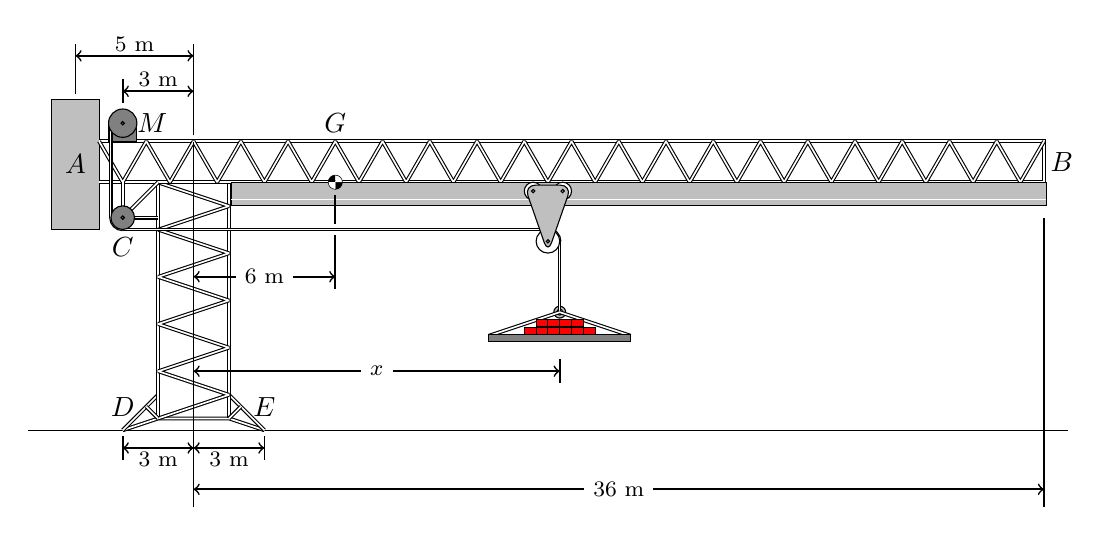
\begin{tikzpicture}[scale=0.3]
        \draw (-4,0) -- (40,0);
        \draw[double] (0,0) -- ++(1.5,0.5)--++(3,0)--++(1.5,-0.5);
        \draw[double] (0,0) -- ++(1.5,1.5) ++(3,0)--++(1.5,-1.5);
        \draw[double] (1.5,0.5) -- ++(0,10)--++(3,0)--++(0,-10);
        \draw[double,join=bevel] (1.5,0.5) -- ++(18.43:3.16) -- ++(161.57:3.16) -- ++(18.43:3.16) -- ++(161.57:3.16) -- ++(18.43:3.16) -- ++(161.57:3.16) -- ++(18.43:3.16) -- ++(161.57:3.16) -- ++(18.43:3.16) -- ++(161.57:3.16);
        \draw[double] (1.5,0.5) -- +(135:0.707);
        \draw[double] (4.5,0.5) -- +(45:0.707);
        \draw[fill=lightgray] (-1,8.5) rectangle (-3,14) node at +(1,-2.75) {$A$};
        \draw[double] (-1,10.5) -- ++(40,0) -- ++(0,1.732) -- ++(-40,0);
        \draw[double,join=bevel] (-1,10.5+1.732) -- ++(-60:2) -- ++(60:2) -- ++(-60:2) -- ++(60:2) -- ++(-60:2) -- ++(60:2) -- ++(-60:2) -- ++(60:2) -- ++(-60:2) -- ++(60:2) -- ++(-60:2) -- ++(60:2) -- ++(-60:2) -- ++(60:2) -- ++(-60:2) -- ++(60:2) -- ++(-60:2) -- ++(60:2) -- ++(-60:2) -- ++(60:2) -- ++(-60:2) -- ++(60:2) -- ++(-60:2) -- ++(60:2) -- ++(-60:2) -- ++(60:2) -- ++(-60:2) -- ++(60:2) -- ++(-60:2) -- ++(60:2) -- ++(-60:2) -- ++(60:2) -- ++(-60:2) -- ++(60:2) -- ++(-60:2) -- ++(60:2) -- ++(-60:2) -- ++(60:2) -- ++(-60:2) -- ++(60:2) node at +(0.75,-1.723/2) {$B$};
        \draw[fill=lightgray] (4.6,10.5) rectangle (39.1,9.5);
        \draw[double] (0,10.5) -- ++(0,-1.5) -- +(1.5,0);
        \draw[double] (0,9) -- +(45:2.121);
        \draw[fill=gray] (-0.6,13) rectangle (0.6,10.5+1.732);
        \draw[fill=lightgray, even odd rule] (18.5,5) circle (0.25) circle (0.125);
        \draw[double distance=0.4] (-0.5,13) -- ++(0,-4) ++(0.5,-0.5) -- ++(18,0) ++(0.5,-0.5) -- ++(0,-3);
        \draw (18,8.55) arc (90:0:0.55);
        \draw[fill=white] (18,8) circle (0.5);
        \draw[color=white] (4.6,9.75) -- (39.1,9.75);
        \draw[fill=white] (18.625,10.125) circle (0.375) +(-1.25,0) circle (0.375);
        \draw[rounded corners, fill=lightgray] (18,7.5) -- (19,10.375) -- ++(-2,0) -- cycle;
        \draw (18,8) circle (0.07);
        \draw (18.625,10.125) circle (0.07) +(-1.25,0) circle (0.07);
        \draw (-0.55,9) arc (180:270:0.55);
        \draw[fill=gray] (0,9) circle (0.5) circle (0.07) node at +(0,-1.25) {$C$};
        \draw[fill=gray] (0,13) circle (0.6) circle (0.07) node at +(1.25,0) {$M$};
        \draw[double] (18.5,5) -- +(3,-1) (18.5,5) -- +(-3,-1);
        \draw[fill=gray] (15.5,4.05) rectangle (21.5,3.755);
        \draw[fill=red] (17,4.06) rectangle +(0.5,0.3);
        \draw[fill=red] (17.5,4.06) rectangle +(0.5,0.3);
        \draw[fill=red] (18,4.06) rectangle +(0.5,0.3);
        \draw[fill=red] (18.5,4.06) rectangle +(0.5,0.3);
        \draw[fill=red] (19,4.06) rectangle +(0.5,0.3);
        \draw[fill=red] (19.5,4.06) rectangle +(0.5,0.3);
        \draw[fill=red] (17.5,4.37) rectangle +(0.5,0.3);
        \draw[fill=red] (18,4.37) rectangle +(0.5,0.3);
        \draw[fill=red] (18.5,4.37) rectangle +(0.5,0.3);
        \draw[fill=red] (19,4.37) rectangle +(0.5,0.3);
        %Dimensions
        \draw[semithick] (0,-0.25) -- +(0,-1) node at +(0,1.25) {$D$} ++(3,-3) -- +(0,3.25+10.5+1.723) ++(3,3) -- +(0,-1) node at +(0,1.25) {$E$} ++(33,-3) -- +(0,12.25);
        \draw[semithick] (3,10.75+1.732) -- (3,13.6+0.25+1+1.5) ++(-3,-1.5) -- +(0,-1);
        \draw[semithick] (-2,14.25) -- (-2,13.6+0.25+1+1.5);
        \draw[semithick] (9,6)--++(0,2.25) ++(0,0.5)--(9,9.95);
        \draw[semithick] (18.5,2) -- +(0,1);
        \fill (9,10.5) -- ++(0.3,0) arc (0:-90:0.3) -- ++(0,0.6) arc (90:180:0.3);
        \fill[white] (9,10.5) -- ++(0.3,0) arc (0:90:0.3) -- ++(0,-0.6) arc (270:180:0.3);
        \draw[very thin] (9,10.5) circle (0.3) node at +(0,2.5) {$G$};
        \draw[semithick, to-to] (0, -0.75) -- +(3,0) node[font=\footnotesize] at +(1.5,-0.5) {3 m};
        \draw[semithick, to-to] (3, -0.75) -- +(3,0) node[font=\footnotesize] at +(1.5,-0.5) {3 m};
        \draw[semithick, to-to] (3, -2.5) -- +(36,0) node[fill=white, font=\footnotesize] at +(18,0) {36 m};
        \draw[semithick, to-to] (3,13.6+0.25+0.5) -- +(-3,0) node[font=\footnotesize] at +(-1.5,0.5) {3 m};
        \draw[semithick, to-to] (3,13.6+0.25+2) -- +(-5,0) node[font=\footnotesize] at +(-2.5,0.5) {5 m};
        \draw[semithick,to-to] (3,6.5) -- +(6,0) node[fill=white, font=\footnotesize] at +(3,0) {6 m};
        \draw[semithick,to-to] (3,2.5) -- +(15.5,0) node[fill=white,font=\footnotesize] at +(7.75,0) {$x$};
    \end{tikzpicture}

    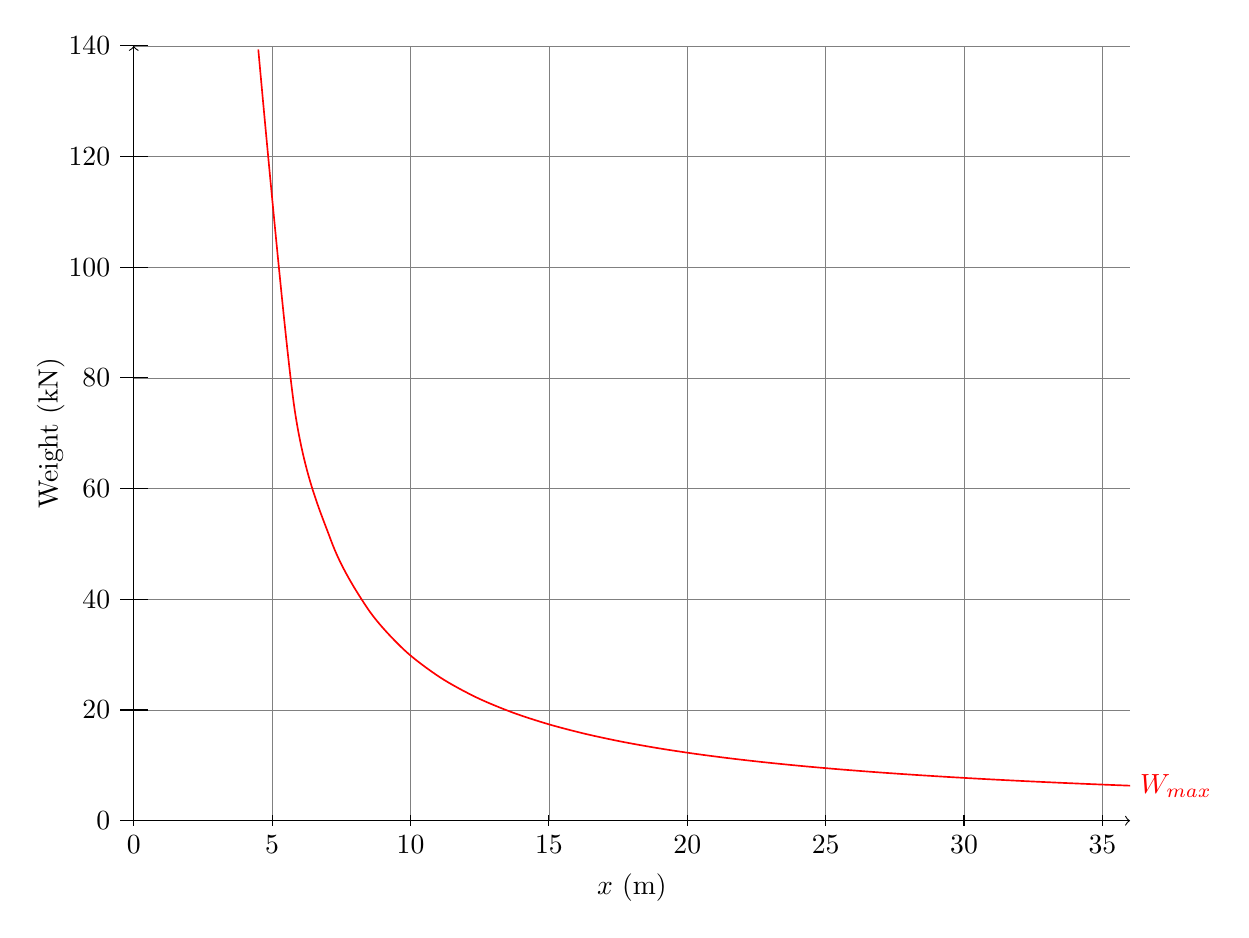
\begin{tikzpicture}[domain=0:36,x=100, y=20, scale=0.1]
        \draw[very thin,color=gray] (0,0) grid[xstep=5,ystep=20] (36,140);
        \foreach \x in {0,5,...,35}
        \draw (\x,1) -- (\x,-1)
        node[anchor=north] {\x};
        \foreach \y in {0,20,...,140}
        \draw (0.5,\y) -- (-0.5,\y)
        node[anchor=east] {\y};
        \draw[->] (0,0) -- (36,0) node at +(-18,-12) {$x$ (m)};
        \draw[->] (0,0) -- (0,140) node[rotate=90] at +(-3,-70) {Weight (kN)};
        \draw[color=red,domain=4.5:36, smooth, semithick] plot (\x,{209/(\x-3)}) node[right] {$W_{max}$};
    \end{tikzpicture}
    \caption{Maximum load of a crane}
    \label{fig:Maximum load of a crane}
\end{figure}

\clearpage

\section{Citations}
\label{sec: Citations}

As one can see in \cite{iso_13849_part1}, functional safety is difficult.

% \nocite means you do not reference the citation in your text 
% but want it included in the bibliography
% BUT: We prefer all sources to be referenced in the text!

\nocite{iso_13849_part1}
\nocite{iso_13849_part2}
\nocite{iso_12100}
\nocite{ISO:online}
\nocite{IEC:online}
\nocite{DIN:online}
\nocite{Isermann2010}
\nocite{francke2015internet}

\section{How To Use Abbreviations}

\glsxtrlong{ASIL}, \glsxtrshort{ASIL}, and \glsxtrfull{ASIL}


\glsxtrshort{C}
\glsxtrshort{CEN}
\glsxtrshort{CENELEC}
\glsxtrshort{DIN}{DIN}
\glsxtrshort{E}{E}
\glsxtrshort{AELV}
\glsxtrshort{ETSI}
\glsxtrshort{EMC}
\glsxtrshort{EN}
\glsxtrshort{F}
\glsxtrshort{FIT}
\glsxtrshort{FMEA}
\glsxtrshort{FuSa}
\glsxtrshort{FSR}
\glsxtrshort{FTA}
\glsxtrshort{FZV}
\glsxtrshort{IEC}
\glsxtrshort{ISO}
\glsxtrshort{KBA}
\glsxtrshort{OEMs}
\glsxtrshort{QM}
\glsxtrshort{S}
\glsxtrshort{StVG}
\glsxtrshort{StVO}
\glsxtrshort{StVZO}
\glsxtrshort{TUEV}
\glsxtrshort{UNECE}
\glsxtrshort{VDA}
\glsxtrshort{BPMN}
\glsxtrshort{FBV}
\glsxtrshort{EU}
\glsxtrshort{EC}

% All hierarchies

\chapter{chapter}
\section{section}
\subsection{subsection}
\subsubsection{subsubsection}
\paragraph{paragraph}
\subparagraph{subparagraph}


